\section{Etude de l'exisant}
   Cette partie concerne le plus sur l'architecture globale des serveurs clouds de \gls{mdi}, leurs évolutions 
   au cours du temps ce qui éclaircirera le besoin de la création du nouveau composant 
   point d entrée.  

    \subsection{Le premier Cloud de MDI}
        Les boîtiers ont la particularité de s’intégrer dans tout type de véhicule et permettent
       l’émission, la réception, le traitement et la représentation de données diverses comme
       l'état de la batterie du véhicule, les données standards, les données du propriétaire du
       véhicule ou des données des capteurs du boîtier même (localisation GPS,
       l’accéléromètre, le gyroscope, la consommation de la batterie ...)et un tas d'autres informations complémentaires.
       Ces données là ont besoin d'être traité pour pouvoir en sortir de l'information utile, d'où le besoin de services divers, regroupés 
       dans un cloud. \\ [0.3cm]
    
         Le CloudConnect - ou \gls{CC} - est le premier cloud fait maison de \gls{mdi} qui englobe un ensemble 
        de services pour les clients. Créé en .., \gls{CC} traite 
        jusqu'à présent un nombre important du traitement des données.
        L'architecture globale de ce cloud est comme le montre  le shema suivant: 

        \begin{figure}[ht]
            \centering
            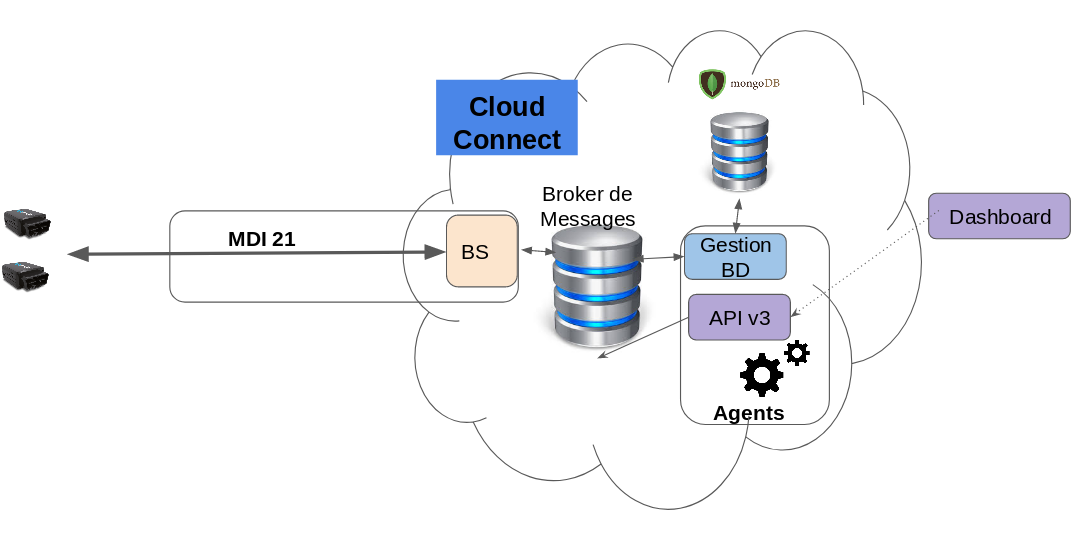
\includegraphics[scale=0.4]{\images/cc.png}
            \caption{L'architecture de CloudConnect - \gls{CC}}
        \end{figure}

        CloudConnect comporte plusieurs composants : 
        \begin{itemize}
            \renewcommand{\labelitemi}{$\bullet$}
            \item  un \gls{BS} qui est le composant d'échange de messages entre le cloud et 
            les OBD. Il consiste le point d'entrée du cloud et qui est le composant à redéfinir.
            \item  un broker de message pour les systèmes Big Data: 
            \item  un ensemble de services qui sont accéder à partir de APIV3 
            \item une base de données pour le stockage des données 
            \item un dashboard pour l affichage des données et l acces visuel 
            des services au clients 
        \end{itemize}
        \vspace{0.2cm}

        \gls{mdi21} est le protocole  ASN1 fait maison, conçu pour la communication entre boîtiers et Cloud.
        Ce protocole sera bien détaillé à la fin de ce chapitre.

    
    \subsection{De \gls{CC} à \gls{CN}}
        Exprimer le besoin du changement d'architecture. 
        Autour de .. \\
        \textbf{Développement des agents :} Un Framework interne est utilisé pour simplifier le développement des différents 
        agents en langage ruby. Ce framework fournit un ensemble de fonctions qui permettent, entre autres, d’accéder au 
        courtier de messages en lecture et en écriture. Concernant les agents à état, le framework ne fournit pas 
        de mécanismes pour simplifier la gestion de leurs états. La gestion de l’état est donc laissée aux développeurs.\\[0.3cm]
        \textbf{Déploiement des agents :} les agents sont exécutés de manière parallèle. En d’autres termes, un agent peut avoir 
        plusieurs instances déployées dans différentes machines. Les différentes instances d’un même agent partagent 
        le traitement du flux des événements mais ne communiquent pas entre eux. Le déploiement ainsi que la maintenance 
        d’un agent se traduisent par une mise-à-jour des fichiers de configuration des machines exécutant l’agent via le logiciel Chef.\\ [0.3cm]

        Solution :  Création d‘un autre Cloud afin de revoir l’architecture logicielle et technique de Cloud 
        Connect afin de simplifier le développement des agents, leurs déploiements ainsi que leurs maintenances et 
        de permettre à des développeurs externes de l’entreprise de coder leurs propres agents.



        \begin{figure}[ht]
            \centering
            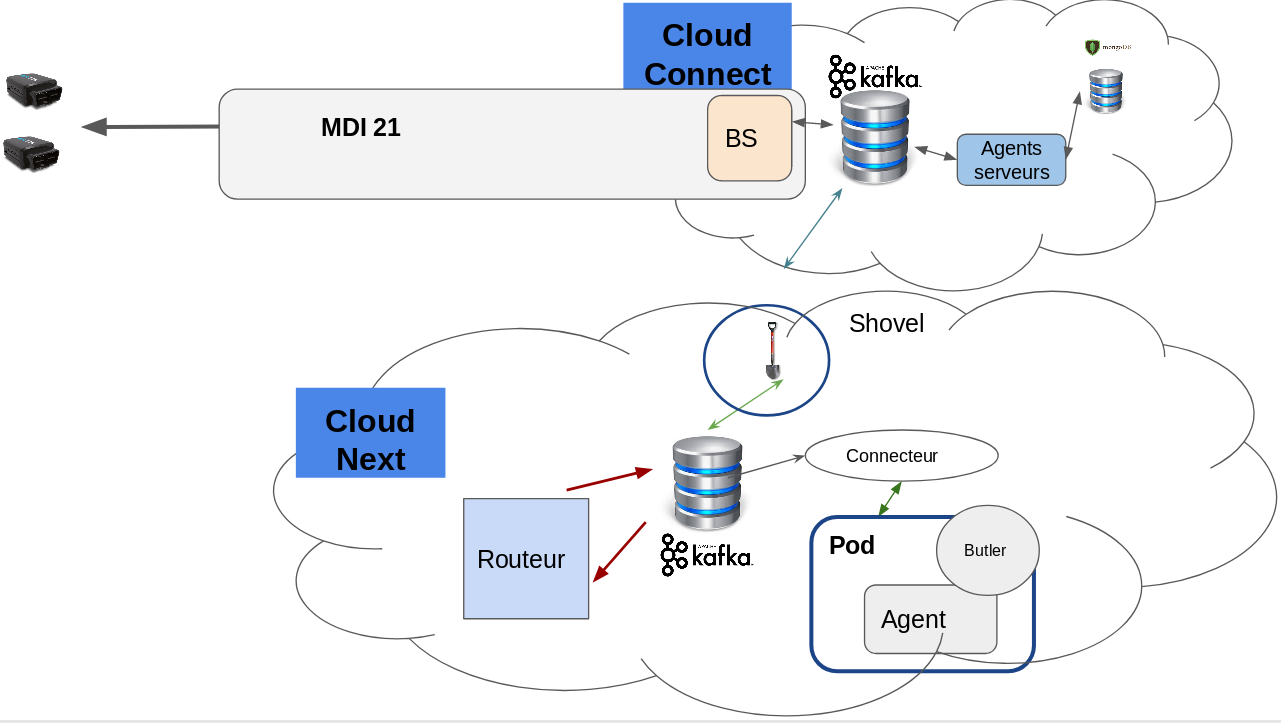
\includegraphics[scale=0.4]{\images/cn.png}
            \caption{L'architecture du cloud avec CloudNext}
        \end{figure}

        \vspace{0.2cm}

       \break

       

        \subsection{Voyons le BS actuel}

        \subsubsection{technologies}
        Redis , Indigen ..., fonctionnalités 
        \subsubsection{Protocole md 21 }
        

        Format des données.
        Format , 

        Track : 
        Message : 
        Presence : 
        


        Paragraphe sur le language Go : 
        Go est un jeune language de programmation système
        fascinant. Ce language compilé hérite des idées des paradigmes de
        programmation impérative et fonctionnelle. Il définit des concepts et
        des règles qui assurent à l'utilisateur des binaires .\\[0.3cm]
       
      
        Le but de cette explication est de montrer la différence considérable
        avec d'autres langages de programmation. Un lecteur intéressé pourra
        apprendre le langage pour plus d'informations.

        MD30, Un nouveau protocol de communication dongle-cloud